\documentclass[10pt,aspectratio=43,mathserif,table]{beamer} 
%  设置为 Beamer 文档类型,设置字体为 10pt,长宽比为16:9,数学字体为 serif 风格
\batchmode

\usepackage{graphicx}
\usepackage{animate}
\usepackage{hyperref}
\usepackage{diagbox} % 表头斜线分区
% 导入一些用到的宏包
\usepackage{amsmath,bm,amsfonts,amssymb,enumerate,epsfig,bbm,calc,color,ifthen,capt-of,multimedia,hyperref}
\usefonttheme{serif}
\usepackage{mathptmx}
\usepackage{xeCJK} %导入中文包
%\setCJKmainfont{SimHei} %字体采用黑体  Microsoft YaHei
%\setmonofont{Courier New}
%\setCJKmainfont[AutoFakeBold = {2.15},ItalicFont={KaiTi}]{SimSun}
%\setCJKfamilyfont{xw}{STXinwei}

%\setsansfont{Microsoft YaHei}

%\setsansfont{Arial}


\usetheme{Berlin} %主题
%\usecolortheme{sustech} %主题颜色

\usepackage[ruled,linesnumbered]{algorithm2e}

\usepackage{fancybox}
\usepackage{xcolor}
% \usepackage{times}
\usepackage{listings}

\usepackage{booktabs}
\usepackage{colortbl}

\newcommand{\Console}{Console}
\lstset{ %
	backgroundcolor=\color{white},   % choose the background color
	basicstyle=\footnotesize\rmfamily,     % size of fonts used for the code
	columns=fullflexible,
	breaklines=true,                 % automatic line breaking only at whitespace
	captionpos=b,                    % sets the caption-position to bottom
	tabsize=4,
	commentstyle=\color{mygreen},    % comment style
	escapeinside={\%*}{*)},          % if you want to add LaTeX within your code
	keywordstyle=\color{blue},       % keyword style
	stringstyle=\color{mymauve}\ttfamily,     % string literal style
	numbers=left, 
	%	frame=single,
	rulesepcolor=\color{red!20!green!20!blue!20},
	% identifierstyle=\color{red},
	language=c
}


\definecolor{mygreen}{rgb}{0,0.6,0}
\definecolor{mymauve}{rgb}{0.58,0,0.82}
\definecolor{mygray}{gray}{.9}
\definecolor{mypink}{rgb}{.99,.91,.95}
\definecolor{mycyan}{cmyk}{.3,0,0,0}

%题目,作者,学校,日期
\title{Transcritical Bifurcation}
%\subtitle{\fontsize{9pt}{14pt}\textbf{跨临界分岔}}
\author{Introducer: Yichen Lu\quad \newline  \newline \quad }
\institute{\fontsize{8pt}{14pt}}
\date{\today}

%学校Logo
%\pgfdeclareimage[height=0.5cm]{sustech-logo}{sustech-logo.pdf}
%\logo{\pgfuseimage{sustech-logo}\hspace*{0.3cm}}

\AtBeginSection[]
{
	\begin{frame}<beamer>
	\frametitle{\textbf{Contents}}
	\tableofcontents[currentsection]
\end{frame}
}
\beamerdefaultoverlayspecification{<+->}
% -----------------------------------------------------------------------------
\begin{document}
% -----------------------------------------------------------------------------

\frame{\titlepage}

% \section[Contents]{}   %目录
% \begin{frame}{Contents}
% \tableofcontents
% \end{frame}

% -----------------------------------------------------------------------------
\section{Concept}

\begin{frame}{Bifurcation}
As parameters are varied,
  \begin{itemize}
    \item Fixed points can be created or destroyed,
    \item or their stability can change (stable $\leftrightarrow$ unstable). 
  \end{itemize}
\end{frame}

\begin{frame}{Transcritical Bifurcation}
  \begin{itemize}
    \item A fixed point must exist for all values of a parameter and can never be destroyed
    \item Such a fixed point may change its stability as the parameter is varied
    \item 
	\begin{figure}
      \centering
      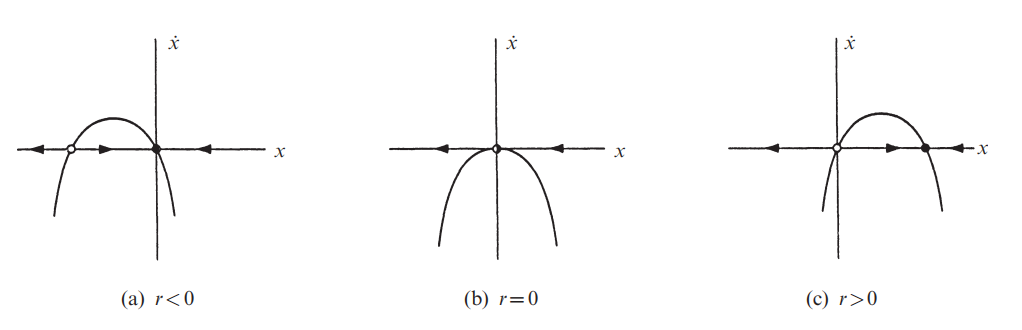
\includegraphics[width=\textwidth]{fig1.png}
    \end{figure}
  \end{itemize}
\end{frame}



\section{Exercises}

\begin{frame}{Exercises 3.2.1}

Sketch all the qualitatively different vector fields that occur as $r$ is varied. Show that a transcritical bifurcation occurs at a critical value of $r$, to be determined. Finally, sketch the bifurcation diagram of fixed points $x^*$ vs. $r$.

Consider the following system of ODEs:

$$\dot{x} = rx + x^2$$

Note that $x = 0$ is a fixed point for all value of $r$


\end{frame}


\begin{frame}
	All the qualitatively different vector fields that occur as $r$ is varied:
	\begin{figure}
		\centering
		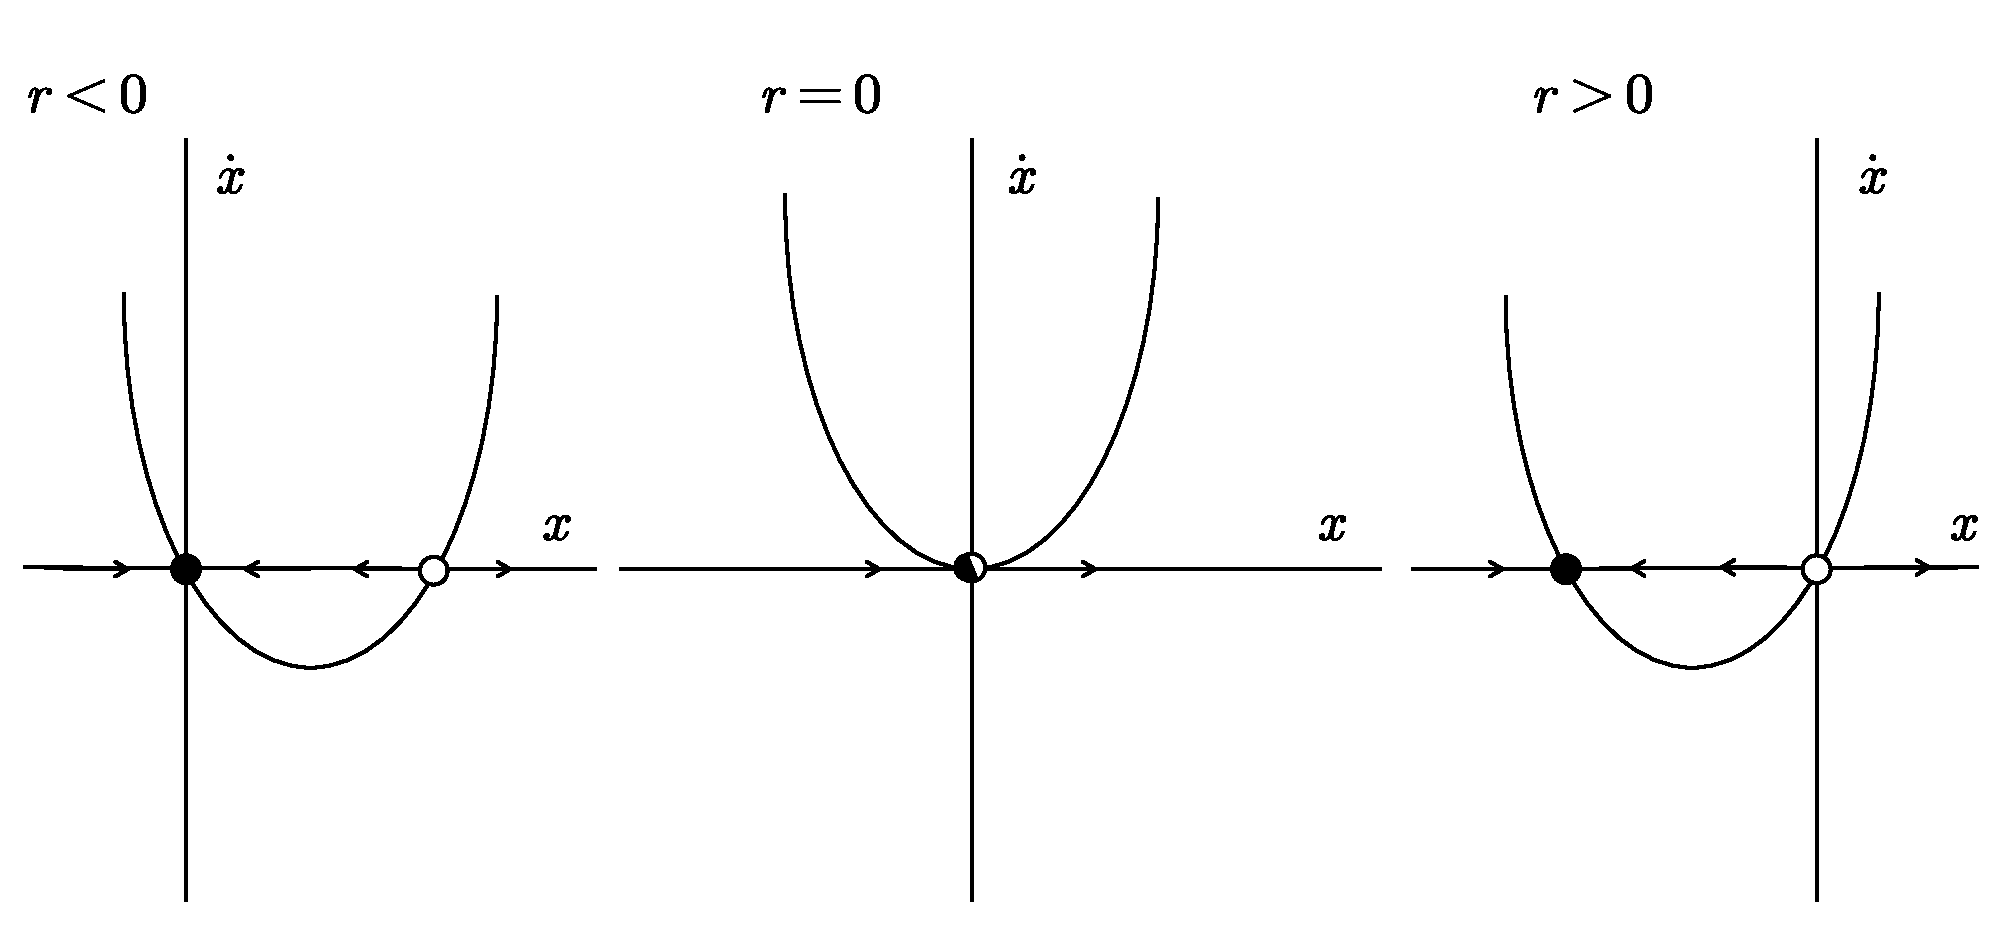
\includegraphics[width=0.8\textwidth]{fig2.pdf}
	\end{figure}
	Transcritical bifurcation occurs at r = 0.
\end{frame}

\begin{frame}
	Bifurcation diagram of fixed points $x^*$ vs. $r$ \ :
	\begin{figure}
		\centering
		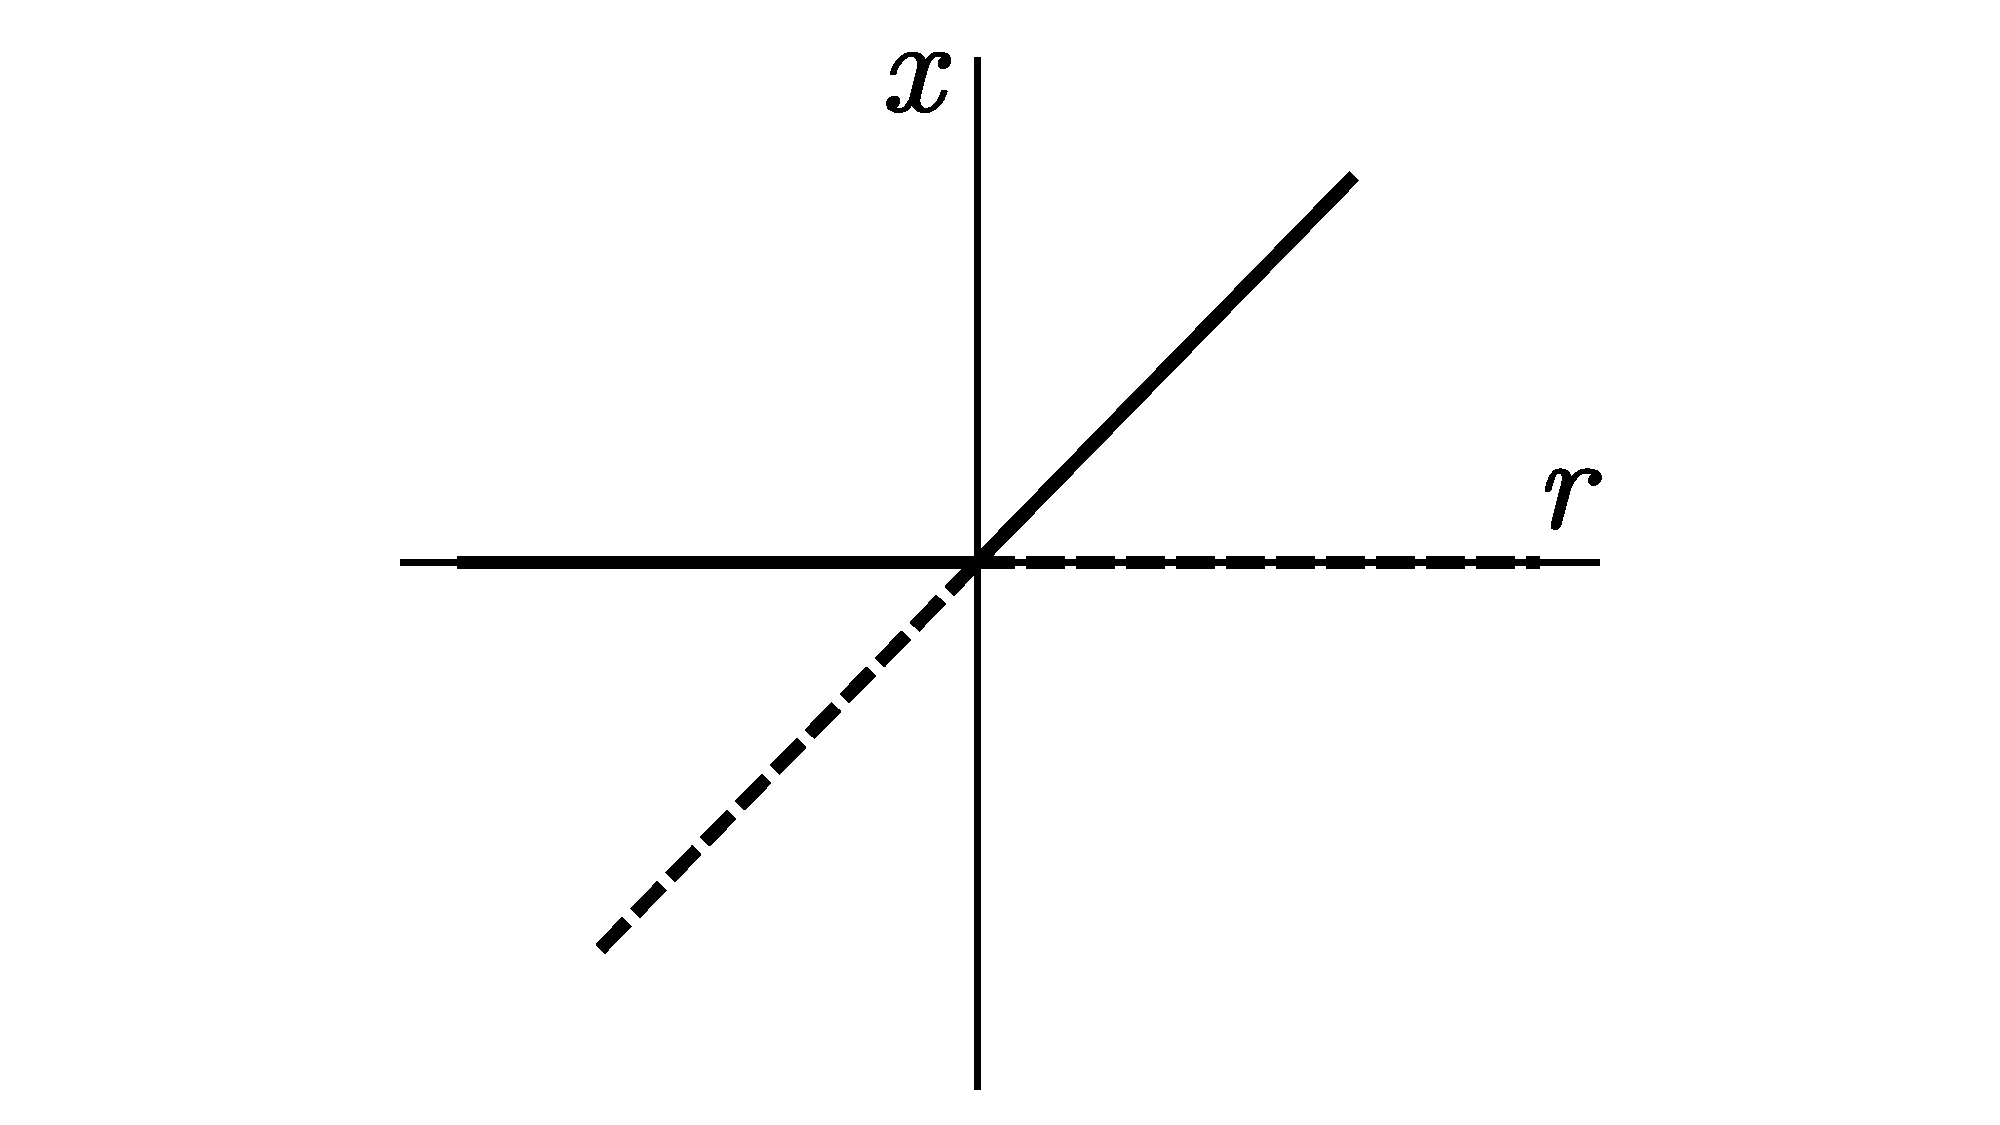
\includegraphics[width=0.85\textwidth]{fig3.pdf}
	\end{figure}
\end{frame}

\begin{frame}{Exercises 3.2.5}
	$$
	A+X \xrightarrow{k_1}\xleftarrow{k_{-1}} 2X \ \ \ X+B\xrightarrow{k_2}C.
	$$
	According to the law of mass action of chemical kinetics, the rate of an elementary reaction is proportional to the product of the concentrations of the reactants. Then the equation for the kinetics of $x$ is
	$$
	\begin{aligned}
		\dot{x}&=k_1ax-k_{-1}x^2-k_2bx\\
		\dot{x}&=(k_1a-k_2b)x-k_{-1}x^2\\
		\dot{x}&=c_1x-c_2x^2\\
	\end{aligned}
	$$
	,where $c_1 = k_1a - k_2b$ and $c_2 = k_{-1}$.

	For $c_1 < 0$, $x^* = 0$ become stable, so $k_1a < k_2b$
\end{frame}

 \begin{frame}
 	 \LARGE \centering Thank you for listening!
 \end{frame}

\end{document}

